\section{Задача 1}

Для линейно упругого материала, представленного на рисунке 1х записать
общий вид матрицы жёсткости в двух декартовых ортогональных системах
координат. Общий вид должен показывать априори равные друг-другу значения
и нулевые значения коэффициентов матриц жёсткости. Охарактеризовать тип
материала.

\begin{figure}[H]
    \begin{center}
        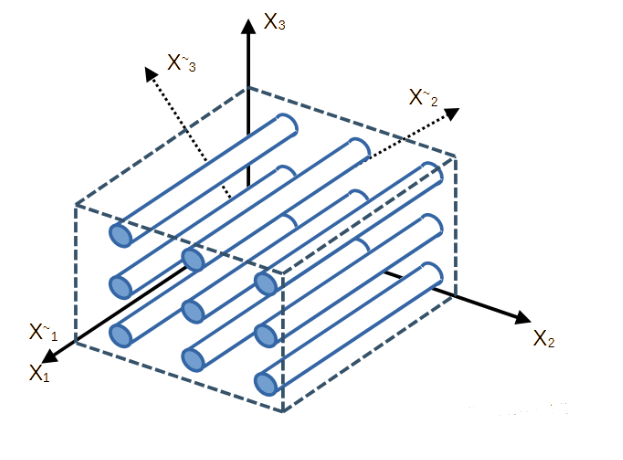
\includegraphics[width = 0.5\linewidth]{pic1.1.PNG}
        \caption{Условие задачи}
        \label{pic1.1}
    \end{center}
\end{figure}

Исходные данные:
\begin{itemize}
    \item СК\_1: $X_1X_2X_3$
    \item СК\_2: $\tilde{X}_2 \tilde{X}_1 \tilde{X}_3$
\end{itemize}

Материал является трансверсально изотропным, он имеет ось симметрии. Количество независимых характеристик упругости равно 5.

\vspace{10pt}
\begin{minipage}{0.5\linewidth}
    \begin{center}
        $X_1X_2X_3$:        
    \end{center}
    \begin{equation*}
        \label{eq1.1}
        C = 
        \begin{bmatrix}
            A & B & B & 0 & 0 & 0
            \\
            B & C & D & 0 & 0 & 0
            \\
            B & D & C & 0 & 0 & 0
            \\
            0 & 0 & 0 & E & 0 & 0
            \\
            0 & 0 & 0 & 0 & E & 0
            \\
            0 & 0 & 0 & 0 & 0 & F
        \end{bmatrix}
    \end{equation*}
\end{minipage}
\begin{minipage}{0.5\linewidth}
    \begin{center}
        $\tilde{X}_2 \tilde{X}_1 \tilde{X}_3$:        
    \end{center}
    \begin{equation*}
        \label{eq1.2}
        C' =
        \begin{bmatrix}
            C & B & D & 0 & 0 & 0
            \\
            B & A & B & 0 & 0 & 0
            \\
            D & B & C & 0 & 0 & 0
            \\
            0 & 0 & 0 & E & 0 & 0
            \\
            0 & 0 & 0 & 0 & F & 0
            \\
            0 & 0 & 0 & 0 & 0 & E
        \end{bmatrix}
    \end{equation*}
\end{minipage}

где:
\begin{equation*}
    \label{eq1.3}
    C = D + 2F
\end{equation*}

откуда:
\begin{equation*}
    \label{eq1.4}
    F = \frac{C - D}{2}
\end{equation*}